\documentclass[fleqn, final]{../styles/unmphythesis}
\usepackage{../styles/qxd}
\renewcommand{\thechapter}{1}
%\newcommand{\thechapter}{1}

\makeindex
\begin{document}
%<*tag>

\renewcommand{\lb}[1]{\label{introduction:#1}}% creates chapter specific labels
\renewcommand{\rf}[1]{\ref{introduction:#1}}% same as before
%\newcommand{\lb}[1]{\label{introduction:#1}}% creates chapter specific labels
%\newcommand{\rf}[1]{\ref{introduction:#1}}% same as before

\chapter{Introduction}
\label{ch:introduction}

%\begin{quote}
%Today, if you have a demanding job for light, you use an optical laser. In the future, if there is a demanding job for atoms, you may be able to use an atom laser.\\[4pt]
%--  Wolfgang Ketterle\ai{Ketterle, Wolfgang}
%\end{quote}
%\url{http://cua.mit.edu/ketterle_group/Projects_1997/atomlaser_97/atomlaser_comm.html}
\section{Motivation}

%After billions of years of evolution since life originated on earth, human being emerge as one of the most wondering and collaborative species, who have come to the point as of today that we work together to understand the quantum nature of matter and use our accumulated knowledge to control the flow of information on microscopic scale for our own purposes. 
%We kill, we conquer, we adapt, we change, we imagine, we love, we give, we steal, we organize, we take, we smile, we write, we educate, we talk, we cheer, and we think, therefore we are. 
%We may indeed need to pass information in the precise units of quanta to be energy-efficient, as the bits of information we rely on in our daily life grow exponential.
%We may indeed need so-called quantum computers to speed up information processing exponentially faster than ever before in order to cope the big mess and the entropy growth we damped to the environment to make ourselves look cool. 

There has been a rapid growth for the demand of processing and distribution of information. 
Our need for information storage increases exponentially over years, we want more secure communication technologies, and we need faster processors to solve complicated problems. 
To conquer these challenges, quantum information science has emerged in recent decades with promises for a new way of handling information~\cite{Nielsen2010a}. 
In quantum information, the minimum unit is called a qubit~\cite{Schumacher1995Quantum}. 
Different from its classical counterpart, a qubit can be a superposition of the traditional binary $ 0 $ and $ 1 $ states of information. 
Quantum information processing can be implemented on the atomic scale, controlled energy-efficiently using single photons, and yield an ultra-precise measurement readout~\cite{DiVincenzo1998}. 
Quantum information processing can guarantee unconditional security based on the non-cloning theorem~\cite{Park1970concept}, and for certain problems, one can compute with an exponential speedup compared to a classical computer~\cite{Deutsch1985,Beckman1996Efficient,Shor1999Polynomial,Grover1996fast}. We can also use these quantum devices to simulate quantum physics itself to help us understand nature in a new way~\cite{Feynman1982Simulating,Lloyd1996Universal,Cirac2012Goals}.

To date, the community has already recognized a number of architectures for the dream quantum devices: solid-state, natural particles such as atoms and ions and other artificial ``quasi-particles" such as atomic-like defects like NV centers~\cite{Aasen2016Milestones,Nayak2008Non,Qi2011}.
While solid-state-based systems need to be fabricated near-perfectly in order to make every individual unit indistinguishable enough to be a good qubit, trapped-ion-- and neutral-atom--based systems provide with identical units already by nature after some isotope selections. 
Engineers are working on making 50 or more identical qubits from scratch~\cite{Preskill2012Quantum} using quantum dots~\cite{Mi2018coherent}, superconductor Josephson junctions~\cite{Kelly2015State,Knight2017IBM}, and defects in solid state materials~\cite{Ondic2017Enhanced}. 
The community of trapped ions and atoms have been working on isolating atoms from an ensemble for high-fidelity and useful controls immunized from the noisy environment~\cite{Zhang2017Observation,Bernien2017Probing,Friis2017Observation}. 
In some cases, the atom-based systems work as a supplemental testbed using large ensembles to study the nature of many-body interactions, to perform quantum simulations, and to discover new technologies to prepare ourselves for the day when other systems can be scaled to a large number of qubits~\cite{Hempel2018Quantum,Komar2016Quantum,Pagano2018Cryogenic,Debnath2018Observation,Tai2017Microscopy,Aidelsburger2015Measuring}.

Of course, atoms and ions, themselves can also be used as the ultimate platform for quantum information processing and precise measurements, given their theoretical low requirement of energy consuming and extremely high efficiency in manipulating one particle~\cite{Deutsch2000Quantum,Saffman2016Quantum,Daley2008Quantum,Bloch2012Quantum,Bermudez2017Assessing,Marti2018Imaging,Zhang2016Precision,Hagemann2014Ultrastable}.
The cost and difficulty of manipulating an atomic system, in some sense, is to simultaneously produce strong and useful interactions with the control or probe field while very weak damaging interactions with the environment. 
That may be the ``Tao" (Dao) of quantum information processing with neutral atoms, as has been emphasized by my supervisor, Prof. Ivan Deutsch, when talking about this topic.
This philosophy may also be true to follow for manipulating qubits based on other systems at large.

One of the foundations of quantum mechanics and a required operation for quantum information processing is quantum measurement.
Although it has been debated since the origin of quantum mechanics, the community of quantum information scientists has developed a deeper appreciation of the quantum nature of measurement using the technologies developed in recent decades.
The community recognizes that a quantum measurement is not just the same as the classical counterpart, in which a measurement is just a readout process. 
A quantum measurement may also change the state of the object in observation~\cite{C.Cohen-Tannoudji1977}.
%In the quantum case, a measurement is an quantum operator, which not only could yield a readout, but also would change the state of the object. 
Using this interesting nature of quantum measurement, one can examine the EPR paradox to test the foundation of quantum mechanics~\cite{Hensen2015Loophole,Giustina2015Significant,Shalm2015Strong}.
Based on this nature of quantum measurement, the famous measurement-based quantum computing approach has also been invented for an attainable of quantum computers~\cite{Briegel2009}. 

In many labs, quantum measurement experiments on the entangling atom-light interface have already been demonstrated with ensembles of atoms confined in an optical dipole trap. 
Since the interaction between atoms and the probe is weak, $10^4$--$10^6$ atoms are used~\cite{Smith2003a,Montano2015Quantum,Smith2012Quantum,Appel2009Mesoscopic,Saffman2009,Puentes2013Planar,Sewell2012Magnetic}.
Our question is, can we implement strong atom-light coupling on quantum interfaces other than in vacuum, or with cavity QED, and apply some quantum measurement and collective state preparation protocols to begin with? 

This dissertation focuses on the theory of dispersive atom-light interactions with a nanophotonic interface. 
We also refer to our physical system, the atom-waveguide hybrid quantum interface, as a quantum data bus, where the state of the input photons can be mapped to the atoms to for state storage and quantum control, and the state of atoms can also be shuffled to the photons for continuous quantum measurement and other applications.


\section{Our toolbox: Atom-waveguide interface}

There has been substantial development in combining cold atoms and with a nanophotonic waveguide. 
Since 1990s or even earlier, theoretical ideas on trapping atoms along a waveguide have been proposed~\cite{Ovchinnikov1991,Bures1999,Barnett2000,Domokos2001,Burke2002,Domokos2002a} and some proof-of-principle experiments have been demonstrated and discussed~\cite{Hinds1999}. The benefits are clear: the strength of the atom-light coupling can be enhanced dramatically using nanophotonic modes compared to the free propagating optical field, and the systems are naturally compatible with current integrated optical systems for immediate applications. 

%After the key issues and some basic properties of dielectric waveguides have been clear, a lot of efforts of the community have been gradually tunneled into the atom traps using tapered optical nanofibers. 
Trapping atoms along a tapered optical nanofiber became one of the dominant platforms for early studies in the field for the following reasons. 
First, relatively speaking, nanofibers are technically easy and economically cheap to fabricate~\cite{Stiebeiner2010}. 
Second, the guided modes have rich structures to support a broad range of applications~\cite{Tong2004,Kien2004,Tong2012}.
The early studies of the tapered optical nanofiber systems ranged from the implementations of atom traps~\cite{Balykin2004,LeKien2004,LeKien2005b,Sague2008,LeKien2008a,Fu2008,Baade2009,LeKien2009c}, to studies of spontaneous emission of trapped atoms and the efficient coupling of the emissions to the fiber~\cite{LeKien2005a,LeKien2007,Kien2007,Kien2008,LeKien2009b}, interactions between atoms mediated by the fiber~\cite{LeKien2005,Sague2007}, fiber modes and photon correlations mediated by the trapped atoms~\cite{Shen2005,LeKien2006,Shen2007,LeKien2008,Chang2008,LeKien2009,Nayak2009a}, to quantum effects for quantum information applications~\cite{LeKien2009a,Nayak2007,Zoubi2010,Zoubi2012}, and the list goes on. 
%Compared to the progress in theoretical studies, experiments really take a while to nail down technical details. 

The first experiments (by Nayak {\it et al.} in 2007) with neutral atoms and a tapered nanofiber were done by confining a cloud of atoms in a magneto-optical trap (MOT)\index{magneto-optical trap} close to a nanofiber, and the nanofiber was used to collect the fluorescence of atoms close by~\cite{Nayak2007,Nayak2008}. 
Despite the simplicity of the system, the fluorescence spectrum exhibited the fingerprint of spontaneous emission coupled to the fiber by a few atoms very close to the fiber surface. 
Once the technique to distinguish a few coupled atoms from the rest of the atom cloud was established, experimental progress to improve the number of trapped atoms and the quality of nanofiber fabrications become easier than ever before. 
In 2010, Rauschenbeutel's group reported about $ 2000 $ cesium atoms on trap with a mean distance to the fiber surface of $ 200 $ nm~\cite{Vetsch2010Optical}. 
They also proposed a dispersive optical interface using a nanofiber and trapped atoms, based on a technique to count atom number with a resolution of a few tens of atoms~\cite{Dawkins2011}. 
In 2012, Kimble's group demonstrated a state-independent trapping technique~\cite{Goban2012,Lacroute2012}. 
In 2014, the number of trapped atoms have been improved to about $ 3000 $ by Polzik's group~\cite{Beguin2014}, with a new technique to count the number of trapped atoms in two-color probes under a resolution below 10 atoms.

In the meantime, the fabrication technique to produce centimeter-long nanofibers with cavity mirrors have been demonstrated~\cite{Keloth2017Fabrication}, which opens the door to trap more atoms with stronger coupling than ever before. 
Techniques and theories of the state-dependent trapping and manipulating atomic states with real and fictitious magnetic fields have also been studied~\cite{LeKien2013,LeKien2013a,LeKien2013b,Schneeweiss2014,Albrecht2016Fictitious}. 
These studies have contributed to the recent experiments on cooling the atom near to the vibrational ground state~\cite{Beguin2017Observation,Meng2017ground}. 
Based on the platform of nanofiber-trapped atoms, optical switches~\cite{OShea2013,Mitsch2014a,LeKien2014}, quantum memory~\cite{Sayrin2015,Gouraud2015Demonstration,Asenjo-Garcia2017Exponential}, optical isolators~\cite{Sayrin2015a}, anti-bunched photon generators~\cite{LeKien2011a,LeKien2011} and other applications have also been discussed in theory and demonstrated in experiments in recent years. 


To further improve the scalability and coupling strength, other waveguide platforms have been proposed for atom-light interfaces during the last a decade or so, especially for waveguides that can be integrated into semiconductor optical circuits using current mature plane photolithographic techniques. 
These waveguides usually have a rectangular-like shape, being suspended or etched on top of a flat substrate. 
Current studies on these waveguides have focused more on the basic properties and system designs. These include studies ranging from the modal selection and design of integrated waveguides~\cite{Fu2007,Lee2013,Stievater2016Modal}, trapping potential calculations~\cite{Barnett2000,Paul2015Push}, decay rate modeling~\cite{Blanco2004Spontaneous,LeKien2016}, new techniques to transport atoms~\cite{Marchant2011}, new material and structures to enhance the coupling~\cite{Chang2009,Salem2010,Hung2013}. 
There has been experimental progresses on trapping atoms using a photonic crystal waveguide from Kimble's group~\cite{Yu2014,Douglas2013,Douglas2015,Paulisch2015}.
But in these nanofabricated systems, the number of trapped atoms is much less than the nanofiber case so far, and their focus seems to observe few- to many-body strong interactions for quantum simulations and other applications~\cite{Manzoni2016Designing,Manzoni2017Simulating}. 

\begin{figure}
\centering\makebox[\textwidth]{
\includegraphics[width=0.99\linewidth]{../media/Figs/TaperedNanofiber_trappingpotential}}
\caption[Trapping potential and optical lattices along a tapered nanofiber.]{(b) Diagram of a tapered-nanofiber-trapped-atoms system, and the trapping potential (a) in the $ xz$ plane sliced at $ y=0 $, and (c) in the $ xy$ plane sliced at trapping sites. 
Two counter-propagating red-detuned laser beams ($ \lambda_{red}=937 $ nm) and two counter-propagating blue-detuned laser beams ($ \lambda_{blue}=636 $ nm) are employed to trap alkali atoms at the lowest potential spots of optical lattices along the $ z $ direction on both sides of the $ x $ axis of a nanofiber. 
The fiber axis is set to be the $ z $ axis.
The trapping points are $220$ nm from the surface of the nanofiber. The radius of the nanofiber is $ a=215 $ nm. Other parameters for calculating the trapping potential can be found in Ref.~\cite{Goban2012}. }\label{fig:nanofibertraps}
\end{figure}

In the optical nanofiber systems, the diameter of the waist is about $ 450 $---$ 500 $ nm, which is a half of the trapping and probe light and only supports the fundamental modes of the fiber. 
Therefore, atoms are trapped in the evanescent field of the trapping and probing lights in the nanofiber region.
Nanofiber traps are usually formed by using red-detuned and blue-detuned guided lights (see Fig.~\ref{fig:nanofibertraps}), where the detuning is relative to the D1 and D2 emission lines of the alkali atoms~\cite{Goban2012,LeKien2004}. 
The red-detuned light pulls the atoms towards the fiber surface, while the blue-detuned light pushes the atoms away from the fiber~\cite{Lacroute2012}. 
Balancing the power of the two, trapping positions can be formed in a certain distance to the fiber surface. 
By using linearly polarized input light beams, the trapping positions can be aligned on both sides of the fiber. 
Furthermore, with one of the colors of the trapping beams (usually the red-detuned one) shined from both ends of the fiber, a standing wave can be formed, which fixes the trapping spots on two chains of optical lattices with a period determined by the half wavelength of the standing wave. 
In this dissertation, we will also study a square waveguide geometry, towards more general integrated waveguides, which can trap atoms with a similar two-color scheme as the nanofiber case. 
See Fig.~\ref{fig:fiberwg_withatoms} for the geometries of the two waveguides we study.

\begin{figure}
\centering\makebox[\textwidth]{
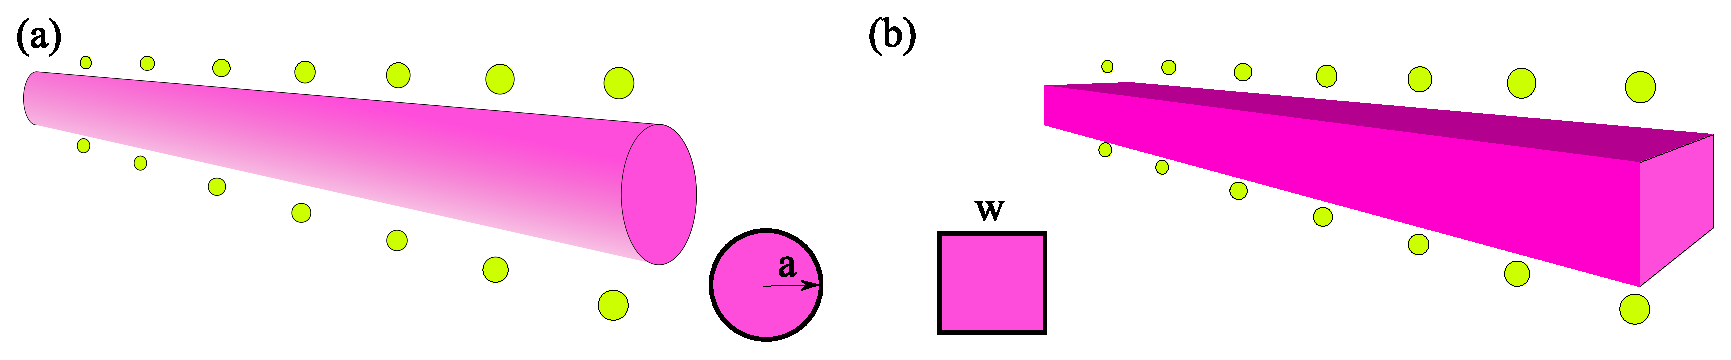
\includegraphics[width=0.89\linewidth]{../media/Figs/fiberwg_withatoms}}
\caption[Trap atoms along a nanofiber and a square waveguide.]{Diagram of Trap atoms along a nanofiber (a) and a square waveguide (b). Insets are the cross sections of the two waveguide geometries.
In this dissertation, we set the radius of the nanofiber as $ a=225 $ nm and the width of the square waveguide as $ w=300 $ nm. }\label{fig:fiberwg_withatoms}
\end{figure}

Comparing these nanophotonic configurations with a free-space atom-light quantum interface, the tight confinement of the waveguide modes provides for a stronger and more uniform coupling between atoms and light~\cite{Qi2016}.
%, and all atoms could be designed to sit in the same field environment, which provides a better mode matching condition. 
In fact, when the free-space trapping and probing configuration is used, there is a tradeoff, for which one most compromises, in the following scenarios~\cite{Baragiola2014}.
%between enhancing the coupling to one atom while trapping less atoms or to trap more atoms yet with a weaker coupling on every atom~\cite{Baragiola2014}.
%as a quantum interface, there is a dilemma to enhance the atom-light coupling. 
If the light is designed to enhance the coupling of atoms at the waist of the laser beam, fewer atoms can be coupled to the light. 
If the light is designed to couple to as many atoms as possible, then the coupling per atom will be weak. %(or optical depth\index{optical depth} (OD) per atom)
%A tradeoff between enhancing the coupling to one atom or to all atoms has to set~\cite{Baragiola2014}.
The waveguide platforms do not have this problem, and one can multiply the coupling strength per atom for all trapped atoms. 
This is a major potential advantage of the nanophotonic systems which can lead to strongly enhanced  cooperativity.

Nevertheless, the nanowaveguide platforms bring in new challenges. 
For example, due to the anisotropy of modes, the atom-light interactions become complicated. 
The alignment-dependent spontaneous emission rates of atoms have been observed in laboratories~\cite{Solano2017Alignment}. 
This new phenomenon hasn't been well considered in many of previous theoretical models in atomic optics, particularly in the context of quantum measurement and quantum control before this study.
What's worse, because of the strong field coupling, there can be strong mechanical oscillations induced by the guided probe on the trapped atoms~\cite{Wuttke2013,Solano2017Dynamics}.
These raise a new dilemma of the benefit over the damage for increasing the effective coupling between atoms and light.

We need new theories to incorporate new phenomena when using the atom-waveguide interfaces.
For quantum information applications, we also need new protocols to best use of the enhanced atom-light coupling while avoiding the disadvantages due to the enhancement itself, which limits the quality of quantum operations. 
As a concrete example, there had not been any theory quantitatively guiding faithful quantum measurements of the internal states of atoms trapped near a nanophotonic waveguides using the guided light field. 
%Without it, atom-waveguide interfaces are rather a blackbox. 
%By understanding the physics code encrypted in the nature of atom-waveguide interfaces, we could potentially gain in-depth insights towards the foundation of quantum mechanics, particularly on matter-light interactions. 
This dissertation focuses on solving these theoretical problems, with applications to quantum measurement and spin squeezing.

%\begin{figure}[ht] % This is generated by inkscape with the option ``PDF+Latex''. The PDF image is in the sub-folder ``images''. The path of the sub-folder is included by adding ``\graphicspath{{images/}}'' to zj.sty.
%   \centering
%   \def\svgwidth{0.85\textwidth} % set the image width, this is optional
%   \input{../Inputs/temperature_gradient.pdf_tex}
%   \caption[Temperature Gradient from a BEC to the Center of the Sun]{Temperature gradient from a BEC to the center of the sun.}
%   \label{fig:temperature_gradient}
%\end{figure}

\section[Quantum measurement, entanglement and spin squeezing with an atomic ensemble]{Quantum measurement, entanglement \\and spin squeezing with an atomic ensemble}
The power of quantum measurement comes from quantum entanglement between the the quantum object to be measured and the probe. 
Below, I will illustrate this statement with a simple example\footnote{Taught by Dr. Ivan H. Deutsch based on Ref.~\cite{Wineland1994Squeezed}.}. Suppose a laser beam in a linearly polarized state $ \ket{\phi_L} $ is shined on an atom that is in a state of $ \ket{\phi_A} =(\ket{\uparrow}+\ket{\downarrow})/\sqrt{2} $. We want to use the laser as a probe to detect the state of the atom, where we have access to the polarization state of the light. The joint state of the atom-polarization system at the initial time $ t=0 $ can be given by
\begin{align}
\ket{\Psi(0)} &=\frac{1}{\sqrt{2}}(\ket{\uparrow}+\ket{\downarrow})\mathbin{\ket{\phi_L}}.
\end{align}
We consider an atom-light interaction defined by an evolution operator, $ \hat{U}(\tau)=e^{i\chi \hat{S}_3 \hat{J_z}\tau} $, where $ \chi $ is the coupling strength between the atom and light, $ \hat{S_3} $ is the Stokes vector operator changing the polarization state of light, and $ \hat{J}_z=\hat{\sigma}_z/2$ is the angular momentum operator for atoms. We will introduce these operators in details for sequential chapters. 
For now, we give that $ \hat{J}_z $ outputs $ +1/2 $ if the atom is in the $ \ket{\uparrow} $ state, and $ -1/2 $ if the atom is in the $ \ket{\downarrow} $ state. 
Then the joint state at time $ \tau $ becomes
\begin{align}
\ket{\Psi(\tau)}&=\frac{1}{\sqrt{2}}\left[\ket{\uparrow}e^{+i\chi \hat{S}_3\tau/2}\ket{\phi_L} 
+\ket{\downarrow}e^{-i\chi \hat{S}_3\tau/2}\ket{\phi_L} \right]\\
&=\frac{1}{\sqrt{2}}\left[\ket{\uparrow}\ket{\phi^1_L} 
+\ket{\downarrow}\ket{\phi^2_L} \right]
\end{align}
where $ \ket{\phi_L^1}=e^{+i\chi \hat{S}_3\tau/2}\ket{\phi_L} $ and $ \ket{\phi_L^2}=e^{-i\chi \hat{S}_3\tau/2}\ket{\phi_L} $ are two polarization states with the polarization axis of the light rotated by $ \pm \chi \tau/2 $, respectively. 
Therefore, the output state of the system is an entangled state. It predicts that, if the polarization state of the light is measured to be rotated by $ +\chi\tau/2 $ from the original state, then the atom is in the $ \ket{\uparrow} $ state. Otherwise, if the light is rotated by $ -\chi\tau/2 $, the atom is in the $ \ket{\downarrow} $ state. 
Therefore, the probe works as a meter for us to access to the state of the atom through the mutual entanglement. 
The sensitivity of the measurement is determined by the rotation angle of the polarization state of the light. 
In other words, to make the measurement outputs more distinguishable, we need to enhance the coupling strength of the bipartite system. 
%\qxd{Put my picture of the meter and measurement here.}

%A quantum state is so fragile that, if you measure it, you also destroy it. We can only gain partial information from one shot of measurement based on the uncertainty principle. 
%If we know the recipe to prepare the quantum state, there are two naive ways to reconstructing the quantum state: to prepare multiple copies of the quantum object and measure them sequentially in different bases; or, to measure the object multiple times by repeating the preparation processes. 
%After the seminar work by Holevo~\cite{Holevo2011Probabilistic}, we now know that the optimal quantum measurement strategy to gain more information with less destructive measurement trials is to prepare multiple copies of the object and measure all of them collectively. Various protocols have been implemented on different quantum systems~\cite{Massar2005Optimal,Derka1998Universal,Jones1994Fundamental}. Particularly, the quantum non-demolition (QND) measurement technique has been implemented on atomic systems~\cite{Smith2003a,Smith2004Continuous}.
%The continuous measurements allowed by QND measurement techniques have paved a solid foundation to recent hot fields including quantum state tomography~\cite{Smith2013,SosaMartinez2016Quantum}, quantum process tomography~\cite{Baldwin2014Quantum}, quantum compressed sensing~\cite{Smith2013} and so on. 

%Moreover, as a result of continuous measurement on a collective state, a squeezed state can be generated. 
Assume we have $ N_A $ atoms initially all prepared in the superposition state as above, $ \ket{\phi_A} = \left[(\ket{\uparrow}+\ket{\downarrow})/\sqrt{2} \right]^{\otimes N_A}$, which is called a spin coherent state\index{state!spin coherent state}.
%Based on the uncertainty principle, the spin coherent state has a possibility distribution for all eigenstate of the ensemble. 
With all atoms coupled with a probe and letting the joint system evolve in time $ \tau $ under the evolution operator introduced above, we replace the single Pauli operator with the collective spin operator $\hat{J}_z=\sum_i^{N_A}\hat{\sigma}_z^{(i)}/2  $. 
The spin coherent state has uncertainty in this spin projection, $\Delta J_z = \sqrt{N_A}/2$.
Upon measuring the probe, the uncertainty after the measurement can be reduced compared to the initial state.
We call this process as spin squeezing. The state generated is called a spin squeezed state\index{state!spin squeezed state}.
The mechanism of measurement-induced squeezing is usually called measurement backaction\index{measurement backaction}.

\begin{figure}[!tpb] % Poincare sphere.
   \centering\makebox[\textwidth]{
   %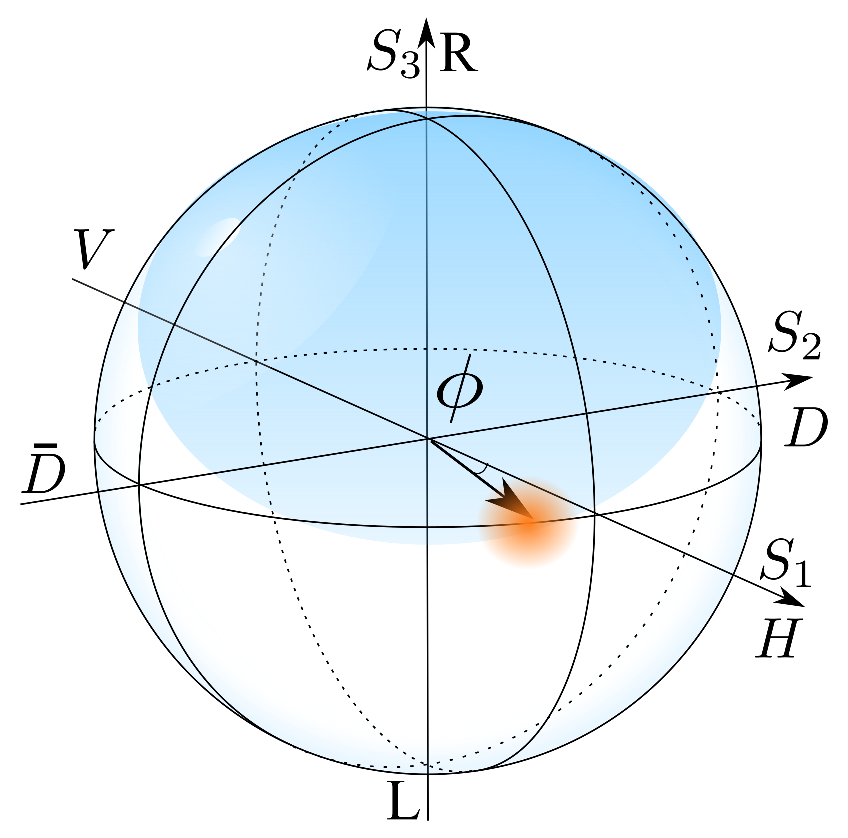
\includegraphics[width=0.55\textwidth]{../media/Figs/poincaresphere_initialS1_Faradayrot_crystal}}
   \begin{minipage}[h]{\linewidth}
    %\begin{tabular}{*{2}{b{0.2\textwidth-2\tabcolsep}}}
     \subfloat[h][]{
       %% This file was created by matlab2tikz.
%
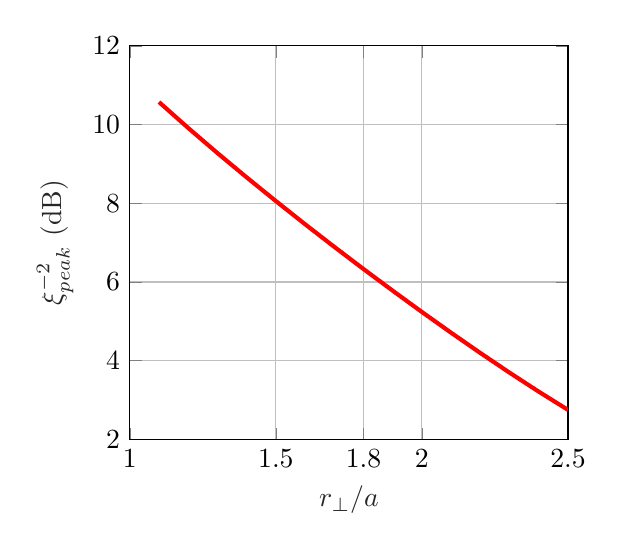
\begin{tikzpicture}

\begin{axis}[%
width=5.565cm,
height=5cm,
at={(0cm,0cm)},
scale only axis,
xmin=1.0000,
xmax=2.5000,
xtick={1.0000,1.5000,1.8000,2.0000,2.5000},
xlabel style={font=\color{white!15!black}},
xlabel={$r_\perp/a$},
ymin=2.0000,
ymax=12.0000,
ylabel style={font=\color{white!15!black}},
ylabel={$\xi^{-2}_{peak}$ (dB)},
axis background/.style={fill=white},
xmajorgrids,
ymajorgrids
]
\addplot [color=red, line width=1.5pt, forget plot]
  table[row sep=crcr]{%
1.1000	10.5712\\
1.2000	9.9128\\
1.3000	9.2762\\
1.4000	8.6588\\
1.5000	8.0571\\
1.6000	7.4685\\
1.7000	6.8935\\
1.8000	6.3307\\
1.9000	5.7799\\
2.0000	5.2394\\
2.1000	4.7118\\
2.2000	4.1974\\
2.3000	3.6980\\
2.4000	3.2157\\
2.5000	2.7531\\
};
\end{axis}
\end{tikzpicture}%
       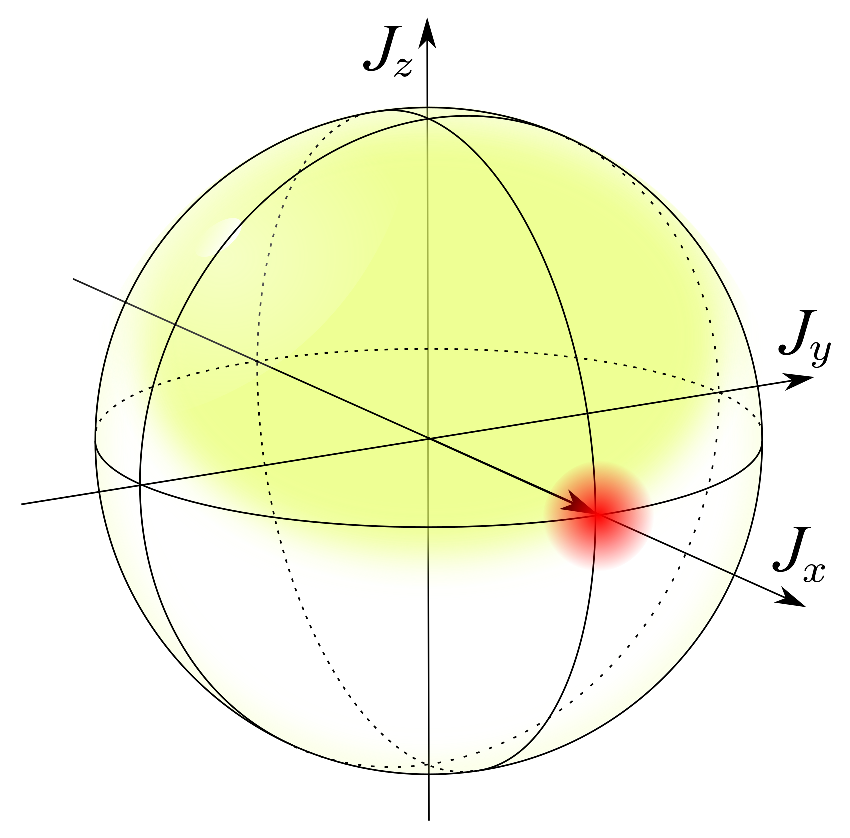
\includegraphics[width=0.3\linewidth]{../media/Figs/blochsphere_initialxJxyz_coherent}
       \label{fig:blochsphere_initialxJxyz_coherent}
       }
       \hfill
     \subfloat[h][]{
         \label{fig:blochsphere_initialxJxyz_squeezed}
         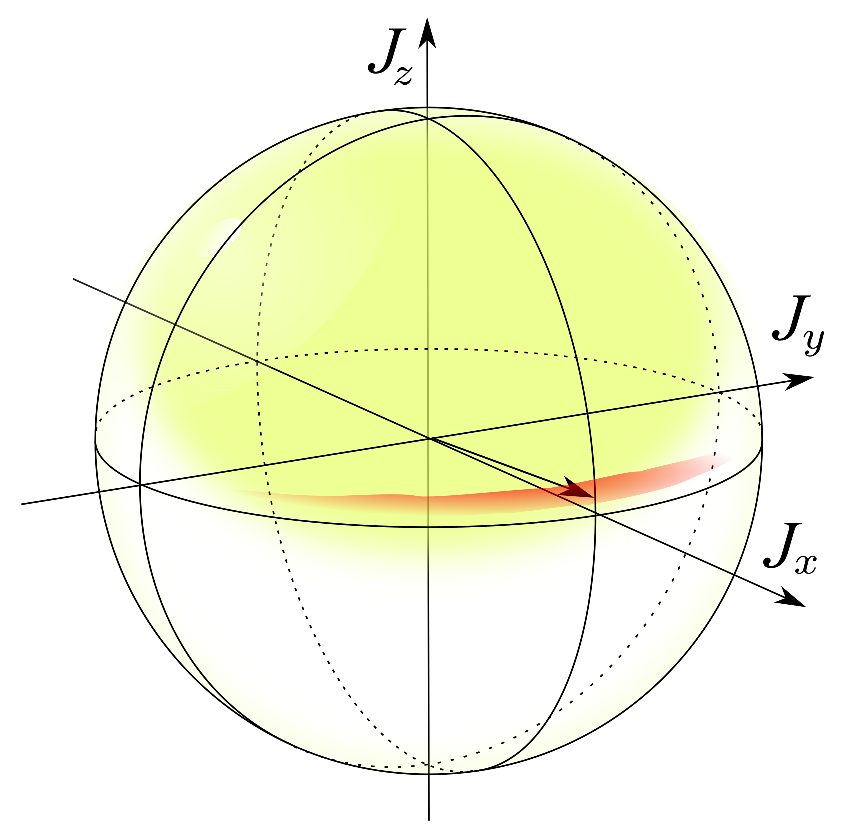
\includegraphics[width=0.3\linewidth]{../media/Figs/blochsphere_initialxJxyz_squeezed}
         %% This file was created by matlab2tikz.
%
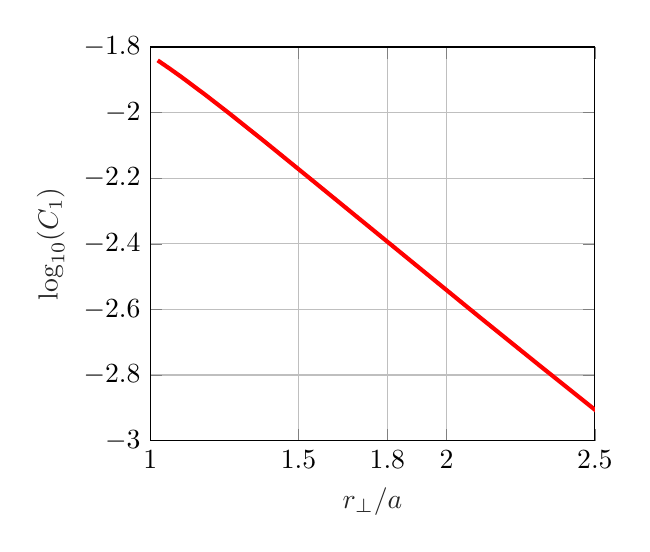
\begin{tikzpicture}

\begin{axis}[%
width=5.647cm,
height=5cm,
at={(0cm,0cm)},
scale only axis,
xmin=1.0000,
xmax=2.5000,
xtick={1.0000,1.5000,1.8000,2.0000,2.5000},
xlabel style={font=\color{white!15!black}},
xlabel={$r_\perp/a$},
ymin=-3.0000,
ymax=-1.8000,
ylabel style={font=\color{white!15!black}},
ylabel={$\log_{10}(C_1)$},
axis background/.style={fill=white},
xmajorgrids,
ymajorgrids
]
\addplot [color=red, line width=1.5pt, forget plot]
  table[row sep=crcr]{%
1.0251	-1.8409\\
1.0653	-1.8658\\
1.1055	-1.8917\\
1.1859	-1.9459\\
1.2663	-2.0022\\
1.3869	-2.0891\\
1.5477	-2.2073\\
2.1106	-2.6230\\
2.3116	-2.7696\\
2.5126	-2.9148\\
};
\end{axis}
\end{tikzpicture}%
         }\hfill
     \subfloat[h][]{
            %% This file was created by matlab2tikz.
%
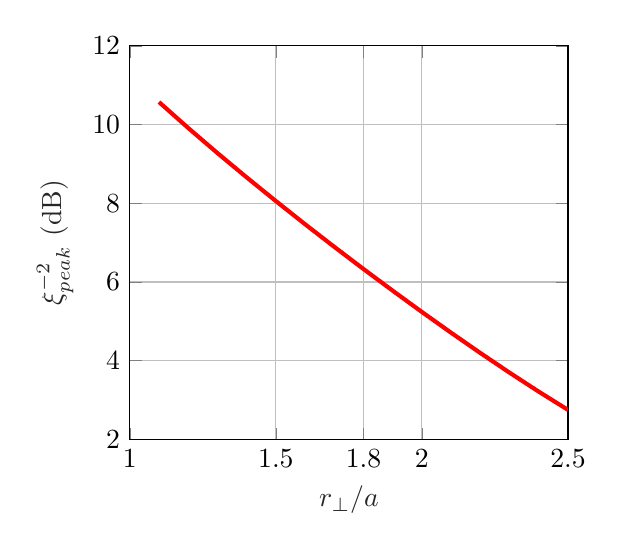
\begin{tikzpicture}

\begin{axis}[%
width=5.565cm,
height=5cm,
at={(0cm,0cm)},
scale only axis,
xmin=1.0000,
xmax=2.5000,
xtick={1.0000,1.5000,1.8000,2.0000,2.5000},
xlabel style={font=\color{white!15!black}},
xlabel={$r_\perp/a$},
ymin=2.0000,
ymax=12.0000,
ylabel style={font=\color{white!15!black}},
ylabel={$\xi^{-2}_{peak}$ (dB)},
axis background/.style={fill=white},
xmajorgrids,
ymajorgrids
]
\addplot [color=red, line width=1.5pt, forget plot]
  table[row sep=crcr]{%
1.1000	10.5712\\
1.2000	9.9128\\
1.3000	9.2762\\
1.4000	8.6588\\
1.5000	8.0571\\
1.6000	7.4685\\
1.7000	6.8935\\
1.8000	6.3307\\
1.9000	5.7799\\
2.0000	5.2394\\
2.1000	4.7118\\
2.2000	4.1974\\
2.3000	3.6980\\
2.4000	3.2157\\
2.5000	2.7531\\
};
\end{axis}
\end{tikzpicture}%
            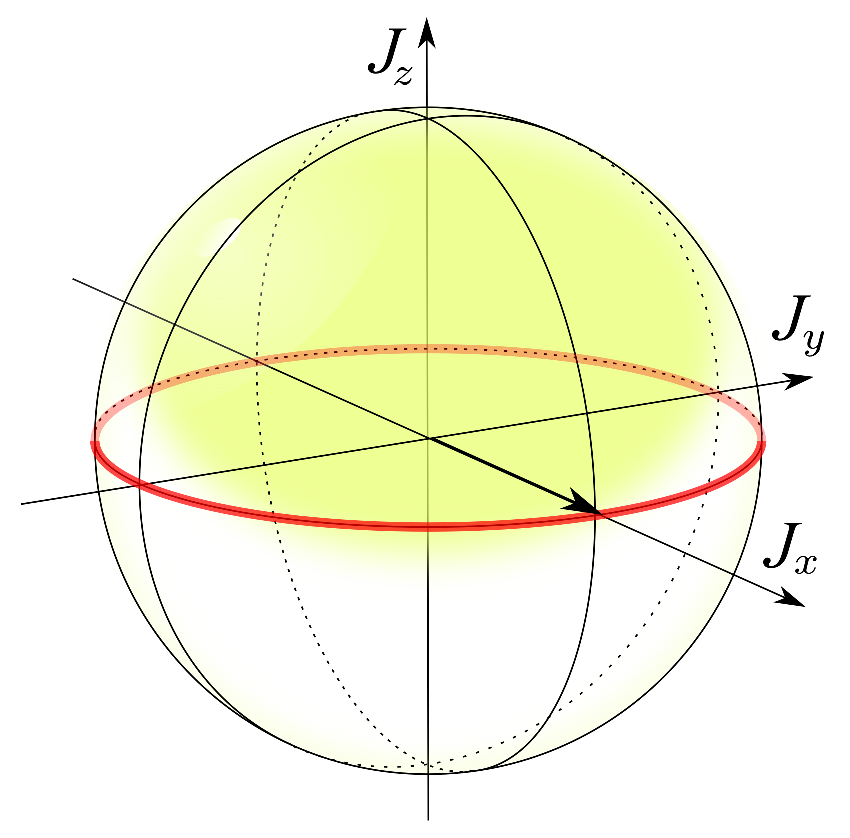
\includegraphics[width=0.3\linewidth]{../media/Figs/blochsphere_initialxJxyz_Dicke}
            \label{fig:blochsphere_initialxJxyz_Dicke}
            }
   \end{minipage}}
   \caption[Coherent state, spin squeezed state and Dicke state on the Bloch sphere.]{Coherent state\index{state!spin coherent state} (a), spin squeezed state\index{state!spin squeezed state} (b) and Dicke state\index{state!Dicke state} (c) on the Bloch sphere\index{Bloch sphere}. 
   The red shadows indicate the probability distributions and uncertainties on the Bloch sphere defined by the collective spin $ \hat{\mathbf{J}} $ vector operator.
   }
   \label{fig:collectivestatesonblochsphere}
\end{figure}


It has been proven by Caves that a squeezed state is crucially useful quantum resource for precise measurements using light~\cite{Caves1981Quantum,Caves1982Quantum}. 
Thus was generalized by Wineland and coworker to employ spin squeezing for Ramsey spectroscopy for use in atomic precision measurement~\cite{Wineland1994Squeezed}.  
In some sense, how much a state is squeezed determines how precise a quantum measurement can be. 
When we plot a squeezed collective state on a Bloch sphere\index{Bloch sphere} that represents the probability distribution of the state, the uncertainty region is squeezed from the initial spin coherent state\index{state!spin coherent state} (see Fig.~\ref{fig:collectivestatesonblochsphere}).  
When the squeezing is weak, the squeezed state\index{state!spin squeezed state} can be regarded as a Gaussian state, which is dominated by pairwise quantum correlations of atoms in the ensemble. 
If the squeezing is on the order of the radius of the Bloch sphere, the collective state become non-Gaussian, which is usually dominated by many-body correlations~\cite{Strobel2014,Dubost2012Efficient}. 
To the extreme, if the state wrap around the Bloch sphere as a line of circle, it is called a Dicke state\index{state!Dicke state}~\cite{Dicke1954}. 
Using a non-Gaussian state for quantum metrology, quantum communications, and in general, for quantum information processing, can offer a better performance than using a Gaussian state~\cite{Strobel2014,Ji2016Quantum,Ghose2007Non,Borelli2016Quantum}.
However, a highly non-Gaussian state of an atomic ensemble is still difficult to produce. 

One of the goals of spin squeezing is to generate a non-Gaussian state, to make a quantum-measurement--induced squeezed state more useful~\cite{Buono2013Quantumness}. 
For an ensemble of atoms, the radius of the Bloch sphere is defined by the total number of atoms and the dimension of the internal states of an atom. 
In addition, the measurement backaction that generates squeezing is proportional to the coupling strength between atoms and probe.
Therefore, the key to generate a highly squeezed state\index{state!spin squeezed state} is to enhance the coupling strength between atoms and light with a given number of atoms. 
We consider the interface of nanophotonic waveguide-trapped atoms towards this goal.




%\section{The philosophy of cooperativity}
%
%For single atom and many.
%
%In general, the evolution of the polarization state of the light in the context of atom-light interaction, characterized by the Stokes vector $\mathbf{S} $ on the \Poincare sphere, may be governed by the following equation~\cite{Deutsch2010a}:
%\begin{align}
%\dt{\mathbf{S}} &= \mathbf{\Theta}\times\mathbf{S}_{in}
%\end{align}
%where the rotating angle vector around $ S_i $ axis can be given by
%\begin{align}
%\Theta_i &\propto \mathrm{OD}\frac{\Gamma}{2\Delta} =N_A\left( \frac{\sigma_0}{A}\right) 
%\left(\frac{\Gamma}{2\Delta}\right),
%\end{align}
%where OD is the total optical depth of the atoms\index{optical depth}, $ N_A $ is the number of atoms, $ \Gamma $ is the spontaneous decay rate of an atom, and $ \Delta $ is the detuning relative to the atomic resonance. 
%We have also defined the OD per atom in terms of the on-resonant cross section of the atom $ \sigma_0 $ and the effective mode area of the optical field at the atom position $ A $ by
%\begin{align}
%\frac{\mathrm{OD}}{N_A} &= \frac{\sigma_0}{A}.
%\end{align}
%Note that, in the free-space trapping case, an effective number of atoms is used to replace $ N_A $, since atoms are not equally coupled to the light.
%In the waveguide case, the formula of OD per atom above applies perfectly. However, there is a hidden secret. 
%
%We realize that the effective mode area can simply written as
%\begin{align}
%A= \frac{A_{\rm interaction}^2}{A_{\rm in}},
%\end{align}
%where $ A_{\rm interaction} $ is the effective area for the interaction depending on the polarization of the light and the internal structure of the atoms, and $ A_{\rm in} $ is the effective mode area of the total local field at the atom positions. 
%In addition, for QND measurements, we will show that the concept of cooperativity per atom, $ C_1 $, is essentially the OD per atom, and we have the following relations 
%\begin{align}
%C_1 =\frac{\kappa}{\gamma_s} \propto \frac{\sigma_0 A_{\rm in}}{A_{\rm interaction}^2},
%\end{align}
%where $ \kappa $ is the measurement strength--indicating the good effect we want, and $ \gamma_s $ is the characteristic photon scattering rate--indicating the damaging effect in the quantum measurement process. 
%Given that $ A_{\rm in} $ is associated with decoherence and such with $\gamma_s  $, we conclude that $ A_{\rm interaction} $ fully defines the useful interaction effects we target for. 
%Both $ A_{\rm in} $ and $ A_{\rm interaction} $ are geometry-dependent, while $ A_{\rm interaction} $ also depends on the internal state of the atoms. 
%Therefore, using nanophotonic waveguides with a given atomic state, one can enhance the atom-light coupling by optimizing the geometry defined by the boundary shape of the waveguide, the atoms' transverse location, the choice of quantization axis, and the polarization direction of the light. 
%In fact, we show protocols that enhance the atom-light coupling by placing the atoms at the azimuthal angle position that has the weakest field to the atom, which is counter-intuitive in the traditional way to think about atom-light coupling. But it is optimal--in the sense that it maximizes the good effect while minimizes the bad effect--and feasible to implement using the nanophotonic waveguides.
%This type of design could potentially solve the dilemma that the mechanical oscillations and other bad effects hindering manipulating atoms grow with the increase of atom-light coupling as people have thought. 
%All of these degrees of freedom of optimization are degenerate in free-space atom-light interfaces and are locked into the geometry-independent effective mode area $ A $--this is one of the main messages we have learned in studying this subject.  
%
%
%Techniques will advance and our knowledge will gain when contradictories are solved.
%We will elucidate these ideas to solve the traditional contradictories with the atom-waveguide interfaces and provide some concrete quantum information protocols in the following chapters. 

%\begin{figure}[ht] %This figure is drew by Inkscape using the very handy tool 'parametric curves'. The fringe is the hard part, and I don't know how to do it elegantly (I just use a combination of 'cheating' methods to generate it). However, there is one command called '\pgfdeclarefunctionalshading' in the tikZ package which could be helpful. But, unfortunately, it requires knowing how to write PostScript codes.
%   \centering
%   \def\svgwidth{0.85\textwidth}
%   \input{../Inputs/double_well_interfer.pdf_tex}
%   \caption[A Double-Well Atom Interferometer]{A double-well atom interferometer~\cite{shin_atom_2004}: (i)~cool the atoms trapped in a single-well potential to form a BEC; (ii)~split the condensate by slowly deforming the single-well potential to a double-well potential; (iii)~apply ac Stark shift potentials to either of the two separated condensates; (iv)~turn off the double-well trapping potential, and let the condensates ballistically expand, overlap, and interfere; and (v)~take an absorption image.}
%   \label{fig:double_well_interfer}
%\end{figure}


\section{Outline of This Dissertation}
In Chapter 2, we introduce the basic properties of the waveguides to be used in modeling polarization spectroscopy measurements. 
These includes the description of polarizations using the Stokes vectors, the properties of the eigenmodes of the waveguides, the dyadic Green's function due to the radiation from atoms near a waveguide and the evolution of the guided modes of waveguides. 
We relate the phase shift of one guided mode of the waveguide with the spontaneous emission rate of the atoms. 
With the changes of the relative phase and amplitudes of two orthogonal guided modes, we can fully describe the polarization transformation of the guided light.
Everything in this chapter is modeled in the classical picture. 
That is, we treat the electromagnetic wave as a classical field and treat atoms as classical electric dipoles.

In Chapter 3, we discuss the modification of the spontaneous emission rate (or decay rate) of atoms by generalizing some of the classical results introduced in Chapter 2 to the quantum regime. 
We introduce the polarizability tensor operators of atoms to describe the hyperfine state of atoms. 
We model the spontaneous emission rates of atoms in the presence of a dielectric waveguide using the Green's function language. 
Using a modal decomposition, we separate the decay rates into the guided and unguided mode components, which are responsible for the polarization transformation of the light and the modification of atomic properties due to the waveguide. 
We use the example of the decay rate calculation for a free dipole in vacuum to introduce the equivalent dipole method for studying the Purcell effect~\cite{Vos2009}.
With this method, we first develop the theory for calculating the modified spontaneous decay rate of classical dipoles due to waveguides without considering the internal structure of atoms. 
Then we generalize this theory to include the internal structure of atoms to calculate the modified decay rates of alkali atoms. 
In the dispersive regime, we find the cases where we can ignore the modification of the decay rates of atoms due to the waveguide.
A geometric explanation of the unique features of waveguide interfaces compared to optical fields in vacuum is given at the end of the chapter to cast some insights on designing a good waveguide geometry for enhancing atom-light coupling. 

Chapter 4 introduces the Hamiltonian, the characteristics of QND measurements and the measurement-induced spin squeezing effect. We define the clock states and the stretched states of individual alkali atoms and some collective states of an atomic ensemble, which will be used for designing our QND measurement and spin squeezing protocols that follow. 

Chapter 5 is based on our publication, Ref.~\cite{Qi2016}, which establishes a general theory to describe atom-light interactions on a nanophotonic waveguide platform (mainly taking the nanofiber dispersive interface as an example) with applications to QND measurement and spin squeezing based on the birefringence interactions. 
We develop an input-output formalism using the Green's function language and solve the light response problem due to atoms near a nanofiber in the Heisenberg-Langevin picture. 
Then we apply our theory to design protocols for atom number counting, QND measurement and spin squeezing by optimizing the choice of quantization axis and finding a magic frequency to cancel noise terms in the interaction Hamiltonian.
We show that $ \sim 4.7 $ dB of squeezing are attainable with $ 2500 $ atoms trapped near a realistic nanofiber, which is a great improvement for small numbers of atoms, and could lead to generation of non-Gaussian states with applications to precise atomic clocks.

Chapter 6 is based on our publication, Ref.~\cite{Qi2017Enhanced}, which is about further enhancement of the cooperativity per atom in the context of Faraday-effect--based QND measurement and spin squeezing with waveguides. 
Such a geometry is useful in the context of creating spin squeezed states\index{state!spin squeezed state} for magnetometry.
We consider both a nanofiber and a square waveguide as examples for designing the protocol. 
We define the cooperativity formula for the QND measurement, which enables us to find the optical geometry to maximize the squeezing effect. 
In order to calculate the spin squeezing parameter, we develop a set of stochastic master equations using microscopic operators and find the relations between our microscopic operators and the collective operators that define the squeezing parameter. We compare the squeezing using the Faraday effect against the birefringence effect, and using nanofibers verse square waveguides. We show the cooperativity we define is the key parameter to guide the design of waveguides and the measurement geometry. We also find the counter-intuitive result that the optimal azimuthal positions of atoms to enhance the squeezing effect is where the local field is the weakest.

We conclude and provide some suggestions for future works in Chapter 7.

%\section{Other Works}
%In addition to the works presented in this dissertation, I have been also working on the following topics during my PhD study at UNM.

%1. Studies on the collective radiation effect of atoms near a nanophotonic waveguide. 
%A summer project has been done and is still on-going in collaboration with Prof. Perry Rice from the Miami University at Ohio. 
%One problem we were worried about for my dissertation study is that the collective photon emission of atoms may be enhanced in presence of a waveguide which may make our problem more complicated~\cite{Asenjo-Garcia2017Atom,Asenjo-Garcia2017Exponential}.
%Through our summer project study, we conclude that, in the dispersive regime, the collective effect can be safely ignored as we wish, and the assumption of pairwise symmetry of atoms can be applied to the calculation of collective spin dynamics. 
%We also worked on some ideas proposed by Prof. Rice to explain collective emission rates of atoms in presence of a nanofiber, which were observed at the laboratories of Prof. Luis Orozco and Prof. Steve Rolston at the University of Maryland. 

%2. To design a probe scheme so that the tensor light shifts are canceled completely for the QND measurement and spin squeezing protocol. 
%In our paper, Ref.~\cite{Qi2017Enhanced}, we assume the tensor light shift of atoms is negligible or has been canceled using experimental techniques developed for the free-space atom-light interfaces~\cite{Montano2015Quantum}. 
%However, no one has done the modeling and simulations for the nanophotonic waveguide cases to-date, in which the decay rates of atoms are state-dependent and are no longer degenerate for different quantum transitions.
%Using the result of Chapter 3, I have developed a draft model for finding a magic frequency to cancel the tensor light shift with two-color probes and for calculating the spin squeezing dynamics including the modification of decay rates. 
%But the math is messy, and no concrete result obtained yet. I plan to finish this project and incorporate my formalism with our colleagues at CQuIC and outside for a general theory of continuous measurement and control using the atom-waveguide interfaces introduced in this dissertation. 


%</tag>
%###################################################################################
\bibliographystyle{../styles/abbrv-alpha-letters-links}
\bibliography{../refs/Archive}
%%%%%%%%%%%%%%%%%%%%%%%%%%%%%%%%%%%%%%%%%%%%%%%%%%%%%%%%%%%%%%%%%%%%%%%%%%%%%%%%%%%%%

\printindex
%\cleardoublepage
%\thispagestyle{plain}
%\phantomsection
%\printindex{ai}{Author Index}
%\chaptermark{Author Index}
%\thispagestyle{plain}
%\printindex{si}{Subject Index}
%\chaptermark{Subject Index}
\end{document}
